\apendice{Esquemas visuais do modelo do Grupo 3}
\label{cap:apendice}

Este apêndice reúne diagramas vetoriais do framework, com foco no objetivo primordial do Grupo 3: segurança como valor, escalabilidade técnica, compliance e retorno econômico.

\renewcommand{\thesection}{\arabic{section}}

\section{Diagrama integrado das cinco dimensões}
\begin{figure}[htb]
\centering
\begin{tikzpicture}[
node distance=1.4cm and 1.8cm,
box/.style={draw, rounded corners=4pt, thick, align=center, minimum width=3.0cm, minimum height=1.1cm, fill=gray!12},
arr/.style={-Latex, thick}
]
\node[box] (a) {Estratégica\\PMBOK 7 + Tailoring};
\node[box, right=of a] (b) {Estrutural\\Platform Design};
\node[box, right=of b] (c) {Engenharia\\Flow Framework};
\node[box, below=of b] (d) {Fiscal\\Lei do Bem};
\node[box, below=of c] (e) {Governança\\VMO + OKRs/OrKRs};
\draw[arr] (a)--(b);
\draw[arr] (b)--(c);
\draw[arr] (c)--(e);
\draw[arr] (d)--(e);
\draw[arr] (a)|-(d);
\draw[arr] (e)-|(a);
\end{tikzpicture}
\caption{Integração sistêmica das cinco dimensões.}
\end{figure}

\section{Mapa mental estratégico revisado}
\begin{figure}[htb]
\centering
\begin{tikzpicture}[
node distance=1.4cm and 1.7cm,
box/.style={draw, rounded corners=4pt, thick, align=center, minimum width=3.3cm, minimum height=1.0cm, fill=gray!12},
arr/.style={-Latex, thick}
]
\node[box, minimum width=4.0cm] (core) {Agro-Secure HaaS\\núcleo de valor};
\node[box, above left=of core] (m1) {Mercado-alvo\\Agro + PMEs};
\node[box, above=of core] (m2) {Oferta\\segurança enterprise};
\node[box, above right=of core] (m3) {Arquitetura\\edge + NFC + SOC};
\node[box, below left=of core] (m4) {Economia\\CAPEX 5,9k / payback 5};
\node[box, below=of core] (m5) {Conformidade\\PD\&I + Lei do Bem};
\node[box, below right=of core] (m6) {3 duplas\\A tração, B operação, C caixa};
\draw[arr] (core)--(m1);
\draw[arr] (core)--(m2);
\draw[arr] (core)--(m3);
\draw[arr] (core)--(m4);
\draw[arr] (core)--(m5);
\draw[arr] (core)--(m6);
\end{tikzpicture}
\caption{Mapa mental estratégico com foco em validação regional, execução e conformidade.}
\end{figure}

\section{Item 2 do anexo --- Business Model Canvas}
\noindent Este bloco consolida visualmente os nove componentes do \textit{Business Model Canvas} aderente ao anexo Agro-Secure.
\begin{figure}[H]
\centering
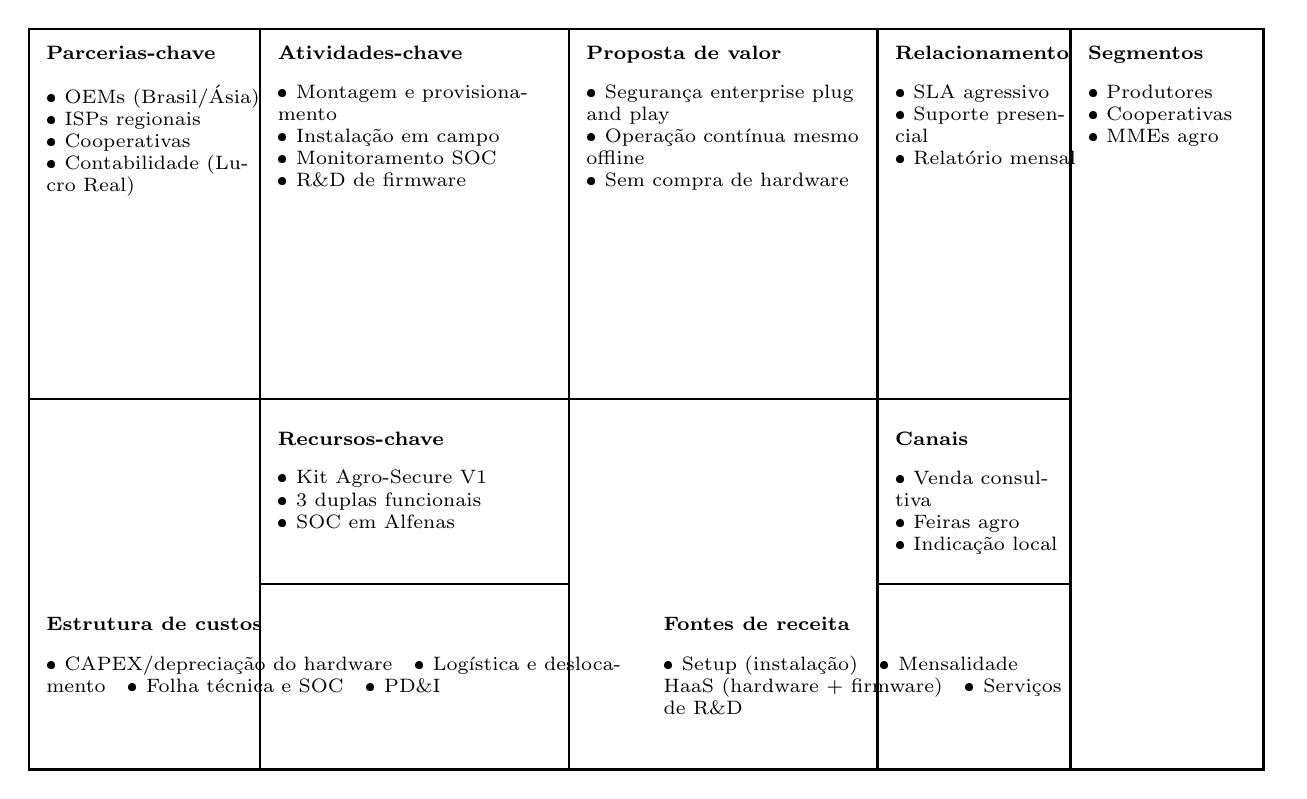
\begin{tikzpicture}[x=0.98cm,y=0.98cm]
\draw[thick] (0,0) rectangle (16,9.6);
\draw[thick] (3,0)--(3,9.6);
\draw[thick] (7,0)--(7,9.6);
\draw[thick] (11,0)--(11,9.6);
\draw[thick] (13.5,0)--(13.5,9.6);
\draw[thick] (0,4.8)--(13.5,4.8);
\draw[thick] (3,2.4)--(7,2.4);
\draw[thick] (11,2.4)--(13.5,2.4);

\node[anchor=north west,font=\bfseries\scriptsize] at (0.1,9.5) {Parcerias-chave};
\node[anchor=north west,font=\scriptsize,align=left,text width=2.8cm] at (0.1,9.0) {\textbullet{} OEMs (Brasil/Ásia)\\\textbullet{} ISPs regionais\\\textbullet{} Cooperativas\\\textbullet{} Contabilidade (Lucro Real)};

\node[anchor=north west,font=\bfseries\scriptsize] at (3.1,9.5) {Atividades-chave};
\node[anchor=north west,font=\scriptsize,align=left,text width=3.8cm] at (3.1,9.0) {\textbullet{} Montagem e provisionamento\\\textbullet{} Instalação em campo\\\textbullet{} Monitoramento SOC\\\textbullet{} R\&D de firmware};

\node[anchor=north west,font=\bfseries\scriptsize] at (3.1,4.5) {Recursos-chave};
\node[anchor=north west,font=\scriptsize,align=left,text width=3.8cm] at (3.1,4.0) {\textbullet{} Kit Agro-Secure V1\\\textbullet{} 3 duplas funcionais\\\textbullet{} SOC em Alfenas};

\node[anchor=north west,font=\bfseries\scriptsize] at (7.1,9.5) {Proposta de valor};
\node[anchor=north west,font=\scriptsize,align=left,text width=3.8cm] at (7.1,9.0) {\textbullet{} Segurança enterprise plug and play\\\textbullet{} Operação contínua mesmo offline\\\textbullet{} Sem compra de hardware};

\node[anchor=north west,font=\bfseries\scriptsize] at (11.1,9.5) {Relacionamento};
\node[anchor=north west,font=\scriptsize,align=left,text width=2.3cm] at (11.1,9.0) {\textbullet{} SLA agressivo\\\textbullet{} Suporte presencial\\\textbullet{} Relatório mensal};

\node[anchor=north west,font=\bfseries\scriptsize] at (11.1,4.5) {Canais};
\node[anchor=north west,font=\scriptsize,align=left,text width=2.3cm] at (11.1,4.0) {\textbullet{} Venda consultiva\\\textbullet{} Feiras agro\\\textbullet{} Indicação local};

\node[anchor=north west,font=\bfseries\scriptsize] at (13.6,9.5) {Segmentos};
\node[anchor=north west,font=\scriptsize,align=left,text width=2.3cm] at (13.6,9.0) {\textbullet{} Produtores\\\textbullet{} Cooperativas\\\textbullet{} MMEs agro};

\node[anchor=north west,font=\bfseries\scriptsize] at (0.1,2.1) {Estrutura de custos};
\node[anchor=north west,font=\scriptsize,align=left,text width=7.6cm] at (0.1,1.6) {\textbullet{} CAPEX/depreciação do hardware\quad \textbullet{} Logística e deslocamento\quad \textbullet{} Folha técnica e SOC\quad \textbullet{} PD\&I};

\node[anchor=north west,font=\bfseries\scriptsize] at (8.1,2.1) {Fontes de receita};
\node[anchor=north west,font=\scriptsize,align=left,text width=5.2cm] at (8.1,1.6) {\textbullet{} Setup (instalação)\quad \textbullet{} Mensalidade HaaS (hardware + firmware)\quad \textbullet{} Serviços de R\&D};
\end{tikzpicture}
\caption{BMC tradicional preenchido com base no anexo Agro-Secure.}
\end{figure}

\section{Item 3 do anexo --- Economia unitária e retorno}
\noindent A economia unitária do modelo HaaS evidencia o equilíbrio entre investimento inicial em hardware e recorrência contratual.
\begin{table}[H]
\centering
\caption{Economia unitária do Kit Agro-Secure V1.}
\begin{tabular}{|p{6.0cm}|p{5.5cm}|}
\hline
\textbf{Indicador} & \textbf{Referência de validação} \\
\hline
CAPEX por kit & R\$ 5.900,00 \\
\hline
Mensalidade recorrente (HaaS) & R\$ 850,00 por cliente/mês \\
\hline
Setup de instalação & R\$ 2.000,00 \\
\hline
Payback do hardware & Aproximadamente mês 5 \\
\hline
Leitura de margem (mês 6 ao 12) & Mensalidade com alta contribuição marginal \\
\hline
\end{tabular}
\end{table}

\section{Item 4 do anexo --- Arquitetura de infraestrutura segura}
\noindent A arquitetura prioriza resiliência local no cliente e monitoramento contínuo remoto via SOC.
\begin{figure}[H]
\centering
\begin{tikzpicture}[
node distance=1.2cm and 1.8cm,
box/.style={draw, rounded corners=4pt, thick, align=center, minimum width=4.0cm, minimum height=1.0cm, fill=gray!12},
arr/.style={-Latex, thick}
]
\node[box] (p) {Perímetro seguro\\Gateway + Firewall + NFC};
\node[box, right=of p] (l) {Processamento local\\Servidor Edge (Home Lab)};
\node[box, right=of l] (i) {Interface física\\Totem/Kiosk};
\node[box, below=of l] (s) {SOC remoto (Alfenas)\\Monitoramento 24/7};
\draw[arr] (p)--(l);
\draw[arr] (l)--(i);
\draw[arr] (s)--(l);
\draw[arr] (s)-| (i);
\end{tikzpicture}
\caption{Arquitetura operacional da oferta HaaS de segurança da informação.}
\end{figure}

\section{Figura 5 (principal) --- Funil de vendas revisado}
\noindent A Figura 5 representa o funil operacional completo, da prospecção por CNAE até a escala regional por cooperativas.
\begin{figure}[H]
\centering
\begin{tikzpicture}
\node[draw,trapezium,trapezium left angle=80,trapezium right angle=100,minimum width=10.6cm,minimum height=1cm,fill=gray!12] (f1) at (0,0) {Prospects qualificados por CNAE (15--20)};
\node[draw,trapezium,trapezium left angle=80,trapezium right angle=100,minimum width=8.9cm,minimum height=1cm,fill=gray!12] (f2) at (0,-1.25) {Diagnóstico técnico e auditoria de risco (7 dias)};
\node[draw,trapezium,trapezium left angle=80,trapezium right angle=100,minimum width=7.2cm,minimum height=1cm,fill=gray!12] (f3) at (0,-2.5) {Pilotos ativos (3 kits / 30 dias)};
\node[draw,trapezium,trapezium left angle=80,trapezium right angle=100,minimum width=5.6cm,minimum height=1cm,fill=gray!12] (f4) at (0,-3.75) {Conversão para HaaS recorrente};
\node[draw,trapezium,trapezium left angle=80,trapezium right angle=100,minimum width=4.0cm,minimum height=1cm,fill=gray!12] (f5) at (0,-5.0) {Escala via cooperativas};
\draw[-Latex,thick] (f1.south)--(f2.north);
\draw[-Latex,thick] (f2.south)--(f3.north);
\draw[-Latex,thick] (f3.south)--(f4.north);
\draw[-Latex,thick] (f4.south)--(f5.north);
\node[draw,rounded corners=2pt,align=left,font=\scriptsize,fill=gray!8,text width=10.9cm] at (0,-6.45) {
\textbf{Papéis por etapa:} Dupla A (segmentação e abordagem consultiva); Dupla B (baseline técnico, implantação e coleta de KPIs); Dupla A+Dupla C (proposta, contrato e viabilidade); Dupla C (governança financeira e escala regional).};
\end{tikzpicture}
\caption{Funil de vendas orientado por validação de valor e protagonismo das três duplas.}
\end{figure}

\section{Item 6 do anexo --- Lei do Bem como barreira de entrada}
\noindent A estratégia fiscal é tratada como vantagem competitiva progressiva, com disciplina de evidências desde o início da operação.
\begin{table}[H]
\centering
\caption{Trilha de conformidade para captura futura dos incentivos da Lei do Bem.}
\begin{tabular}{|p{4.5cm}|p{7.0cm}|}
\hline
\textbf{Eixo} & \textbf{Implementação prática} \\
\hline
Documentação rigorosa & Timesheets, backlog [PD\&I], registro de falhas técnicas e relatórios de incerteza desde o dia 1. \\
\hline
Separação do inovador vs rotineiro & Distinção entre instalação operacional e desenvolvimento de firmware/orquestração offline. \\
\hline
Preparação para Lucro Real & Estruturação contábil e técnica para migração no momento de maturidade econômica (meta: ano 3). \\
\hline
Otimização fiscal esperada & Potencial de abatimento entre 60\% e 80\% sobre dispêndios elegíveis de PD\&I. \\
\hline
\end{tabular}
\end{table}

\section{Item 7 do anexo --- Arquitetura e componentes do kit}
\noindent A tabela a seguir explicita os componentes físicos mínimos para execução do modelo em campo com robustez operacional.
\begin{table}[H]
\centering
\caption{Composição técnica do Kit Agro-Secure V1 e função operacional.}
\begin{tabular}{|p{3.3cm}|p{5.1cm}|p{3.2cm}|}
\hline
\textbf{Componente} & \textbf{Função na operação} & \textbf{Custo médio} \\
\hline
Servidor Edge & Processamento local, persistência offline e sincronização segura de dados críticos. & R\$ 2.100,00 \\
\hline
Gateway de borda & Firewall primário, VPN e proteção do perímetro de rede local. & R\$ 650,00 \\
\hline
Totem NFC & Controle de acesso operacional sem uso de credenciais frágeis ou pendrives. & R\$ 1.500,00 \\
\hline
Nobreak senoidal & Proteção contra oscilações elétricas e continuidade da infraestrutura. & R\$ 1.200,00 \\
\hline
Miscelânea de instalação & Cabeamento, conectores e elementos de fixação/proteção do ambiente. & R\$ 450,00 \\
\hline
\textbf{CAPEX total por kit} & \textbf{Infraestrutura completa em comodato HaaS} & \textbf{R\$ 5.900,00} \\
\hline
\end{tabular}
\end{table}

\section{Painel estatístico do agronegócio mineiro (2024--2026)}
\noindent Esta seção consolida os dados macroeconômicos, cooperativistas e de risco cibernético utilizados para sustentar a viabilidade do modelo HaaS no Sul de Minas.

\begin{table}[H]
\centering
\caption{Indicadores macroeconômicos de Minas Gerais com impacto na tese Agro-Secure.}
\begin{tabular}{|p{6.4cm}|p{5.1cm}|}
\hline
\textbf{Indicador (2025)} & \textbf{Valor} \\
\hline
Receita de exportação do estado & US\$ 18,1 bilhões \\
\hline
Participação do agro nas exportações mineiras & 43,7\% \\
\hline
VBP agropecuário total de Minas Gerais & R\$ 171,80 bilhões \\
\hline
VBP do café em Minas Gerais & R\$ 57,52 bilhões \\
\hline
VBP do leite em Minas Gerais & R\$ 26,73 bilhões \\
\hline
Participação de Minas no café nacional & 54\% \\
\hline
\end{tabular}
\end{table}

\begin{table}[H]
\centering
\caption{Base cooperativista estratégica no Sul de Minas.}
\begin{tabular}{|p{2.6cm}|p{3.3cm}|p{2.9cm}|p{3.0cm}|}
\hline
\textbf{Cooperativa} & \textbf{Faturamento} & \textbf{Volume de café} & \textbf{Base de cooperados} \\
\hline
Cooxupé & R\$ 10,7 bilhões & 6,1 milhões de sacas & \textasciitilde 18.000 famílias \\
\hline
Minasul & Consolidado 2025 & 1,8 milhão de sacas (recebido) & 9.000+ cooperados \\
\hline
Cocatrel & R\$ 3,45 bilhões & 1,83 milhão de sacas & Base Sul de Minas \\
\hline
\end{tabular}
\end{table}

\begin{table}[H]
\centering
\caption{Indicadores de infraestrutura e cibersegurança com efeito direto na viabilidade.}
\begin{tabular}{|p{6.4cm}|p{5.1cm}|}
\hline
\textbf{Variável de risco/operação} & \textbf{Valor de referência} \\
\hline
Produtores com internet de qualidade (MG) & 17\% \\
\hline
Ataques cibernéticos no agro brasileiro (2025) & 39.034 \\
\hline
Média mensal de tentativas de ataque (2025) & 3,2 mil/mês \\
\hline
Participação estimada de ransomware nos incidentes & $>$50\% \\
\hline
Retração estimada do crédito rural em 2025 & -16\% \\
\hline
\end{tabular}
\end{table}

\section{Gráficos estratégicos (pizza, radar e barras)}

\begin{figure}[H]
\centering
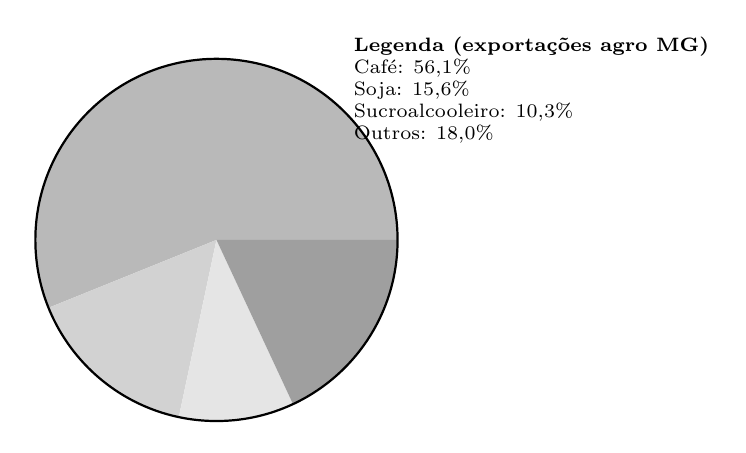
\begin{tikzpicture}[scale=1.0]
\def\r{2.3}
\fill[gray!55] (0,0) -- (0:\r) arc (0:202:\r) -- cycle;
\fill[gray!35] (0,0) -- (202:\r) arc (202:258:\r) -- cycle;
\fill[gray!20] (0,0) -- (258:\r) arc (258:295:\r) -- cycle;
\fill[gray!75] (0,0) -- (295:\r) arc (295:360:\r) -- cycle;
\draw[thick] (0,0) circle (\r);
\node[font=\scriptsize,align=left] at (4.0,1.9) {\textbf{Legenda (exportações agro MG)}\\Café: 56,1\%\\Soja: 15,6\%\\Sucroalcooleiro: 10,3\%\\Outros: 18,0\%};
\end{tikzpicture}
\caption{Gráfico de pizza da composição percentual das exportações agro de Minas Gerais.}
\end{figure}

\begin{figure}[H]
\centering
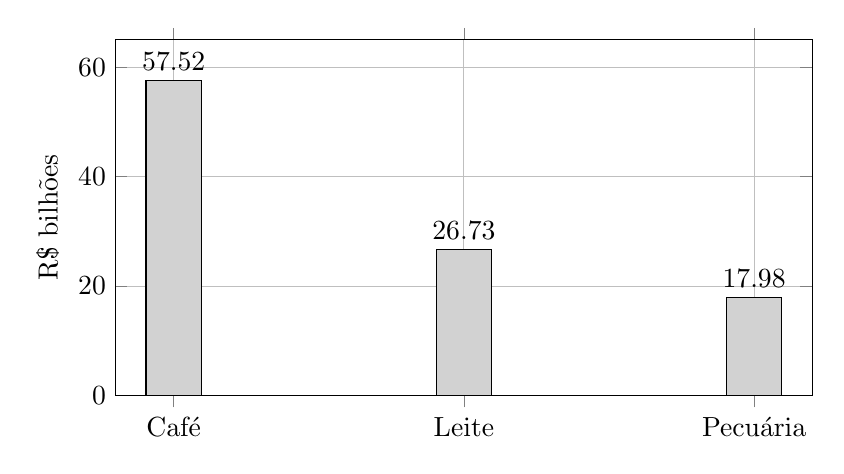
\begin{tikzpicture}
\begin{axis}[
    ybar,
    width=0.86\textwidth,
    height=6.1cm,
    ymin=0,
    ymax=65,
    ylabel={R\$ bilhões},
    symbolic x coords={Café,Leite,Pecuária},
    xtick=data,
    nodes near coords,
    nodes near coords align={vertical},
    bar width=20pt,
    grid=major
]
\addplot[fill=gray!35] coordinates {(Café,57.52) (Leite,26.73) (Pecuária,17.98)};
\end{axis}
\end{tikzpicture}
\caption{Gráfico de barras do VBP mineiro por cadeias relevantes para a tese Agro-Secure.}
\end{figure}

\begin{figure}[H]
\centering
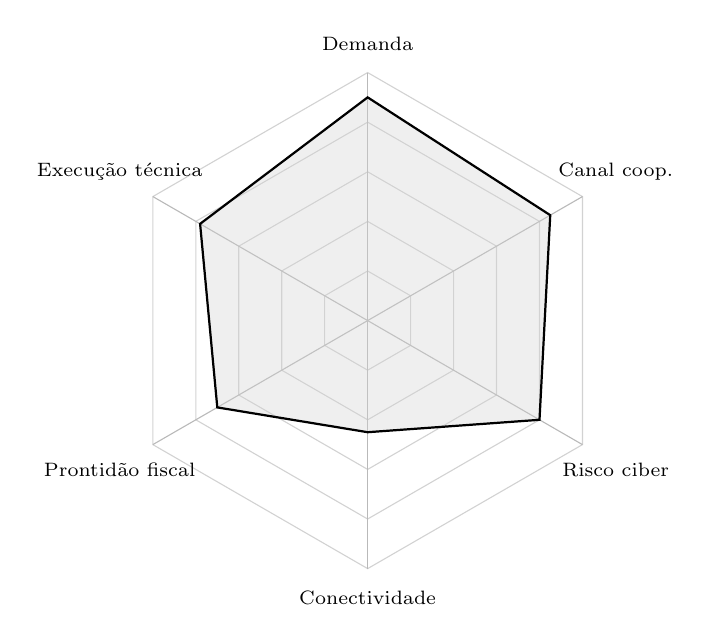
\begin{tikzpicture}[scale=1.05]
\def\R{3.0}
% grade hexagonal
\foreach \k in {0.2,0.4,0.6,0.8,1.0}{
  \draw[gray!35] ({\k*\R*cos(90)},{\k*\R*sin(90)}) -- ({\k*\R*cos(30)},{\k*\R*sin(30)}) -- ({\k*\R*cos(-30)},{\k*\R*sin(-30)}) -- ({\k*\R*cos(-90)},{\k*\R*sin(-90)}) -- ({\k*\R*cos(-150)},{\k*\R*sin(-150)}) -- ({\k*\R*cos(150)},{\k*\R*sin(150)}) -- cycle;
}
% eixos
\foreach \a in {90,30,-30,-90,-150,150}{
  \draw[gray!55] (0,0) -- ({\R*cos(\a)},{\R*sin(\a)});
}
% polígono dos dados (90,85,80,45,70,78)
\draw[thick,fill=gray!35,fill opacity=0.35]
({0.90*\R*cos(90)},{0.90*\R*sin(90)}) --
({0.85*\R*cos(30)},{0.85*\R*sin(30)}) --
({0.80*\R*cos(-30)},{0.80*\R*sin(-30)}) --
({0.45*\R*cos(-90)},{0.45*\R*sin(-90)}) --
({0.70*\R*cos(-150)},{0.70*\R*sin(-150)}) --
({0.78*\R*cos(150)},{0.78*\R*sin(150)}) -- cycle;
% rótulos
\node[font=\scriptsize,align=center] at (0,3.35) {Demanda};
\node[font=\scriptsize,align=left] at (3.0,1.8) {Canal coop.};
\node[font=\scriptsize,align=left] at (3.0,-1.8) {Risco ciber};
\node[font=\scriptsize,align=center] at (0,-3.35) {Conectividade};
\node[font=\scriptsize,align=right] at (-3.0,-1.8) {Prontidão fiscal};
\node[font=\scriptsize,align=right] at (-3.0,1.8) {Execução técnica};
\end{tikzpicture}
\caption{Radar de prontidão estratégica do modelo HaaS no Sul de Minas (escala 0--100).}
\end{figure}

\section{Curvas de ROI acumulado da validação}
\begin{equation}
\mathrm{ROI}(\%) = \frac{\text{Benefício anual esperado} - \text{Investimento total}}{\text{Investimento total}}\times 100
\end{equation}

\begin{figure}[H]
\centering
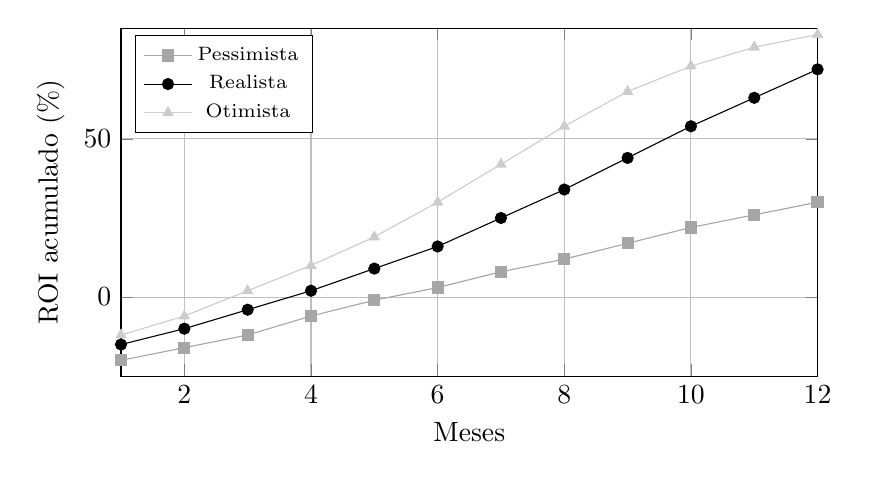
\begin{tikzpicture}
\begin{axis}[width=0.86\textwidth,height=6cm,xlabel={Meses},ylabel={ROI acumulado (\%)},xmin=1,xmax=12,ymin=-25,ymax=85,grid=major,legend style={at={(0.02,0.98)},anchor=north west,font=\scriptsize}]
\addplot[color=gray!70,mark=square*] coordinates {(1,-20) (2,-16) (3,-12) (4,-6) (5,-1) (6,3) (7,8) (8,12) (9,17) (10,22) (11,26) (12,30)};
\addlegendentry{Pessimista}
\addplot[color=black,mark=*] coordinates {(1,-15) (2,-10) (3,-4) (4,2) (5,9) (6,16) (7,25) (8,34) (9,44) (10,54) (11,63) (12,72)};
\addlegendentry{Realista}
\addplot[color=gray!40,mark=triangle*] coordinates {(1,-12) (2,-6) (3,2) (4,10) (5,19) (6,30) (7,42) (8,54) (9,65) (10,73) (11,79) (12,83)};
\addlegendentry{Otimista}
\end{axis}
\end{tikzpicture}
\caption{Curvas de ROI acumulado por cenário para suporte à decisão de escala.}
\end{figure}